\documentclass[11pt,UTF8]{ctexart}
\title{低粘性流体中间夹高粘性泊肃叶流体}
\author{马坤}
\date{2019.10.16}
\usepackage{amsmath}
\usepackage{graphicx}
\usepackage{caption}
\usepackage{subcaption}
\usepackage[left=1in, right=1in, top=1in, bottom=1in]{geometry}
\begin{document}
    \maketitle
    \par{本实验选用的二维泊肃叶流作为模拟的对象,选取$U_0=0.1$
    作为流体的峰值速度,上下固体板速度均为0。模拟的范围为$H=L=1$
    的矩形区域,流体密度均是$\rho_0=1$,由于是泊肃叶流,所以有其
    对应的控制方程与解,形式如下:}
    $$
    \frac{\partial p}{\partial x}=\frac{\partial}{\partial y}(\eta\frac{\partial u}{\partial y}).\eqno(1)
    $$$$
    u = 4U_0\frac{y}{H}(1-\frac{y}{H}).\eqno(2)
    $$
    \par{低粘性流体中间夹高粘性流体,我们采用示性函数$\phi$来
    表示,其定义如下:
    $$
    \phi =
    \begin{cases}
        \frac{1}{2}[\tanh{\frac{y-H/3}{W}}+1],\text{y$\leq$H/2}\\
        \frac{1}{2}[-\tanh{\frac{y-2H/3}{W}}+1],\text{y$>$H/2}
    \end{cases}
    $$
    在大粘性流体中为1,在小粘性流体中为0,在边界
    $(y=H/3,y=2H/3)$上为0.5。数值模拟中,我们分别选取了
    $W=1,W=0.1$的情况。利用$\phi$可以定义流体各处的粘性系数(无维度化后的结果,其与真实的粘性系数节差一个$\eta_l$):
    $$\eta = 1+\frac{\eta_s}{\eta_l}\phi-\phi.\eqno(3)$$
    模拟中我们均采取了高低粘性系数流体的粘性比为50,并取
    $Re=500$使得粘性系数最大值与黄老师的数值匹配。}
    \par{泊肃叶流体中力和压强梯度有一个替代的关系:
    $F = -\frac{\partial p}{\partial x}$,于是我们将$(2)(3)$
    代入$(1)$就可以计算得到力的表达式:
    $$
    F = -\eta \frac{\partial^2 u}{\partial y^2} - \frac{\partial \eta}{\partial y}\frac{\partial u}{\partial y}
    $$
    将上述表达式代入,有$F$的精确表达式。其中图$1$我们给出$W=0.1$时的$F(y)$的图像。
    \begin{figure}[h]
        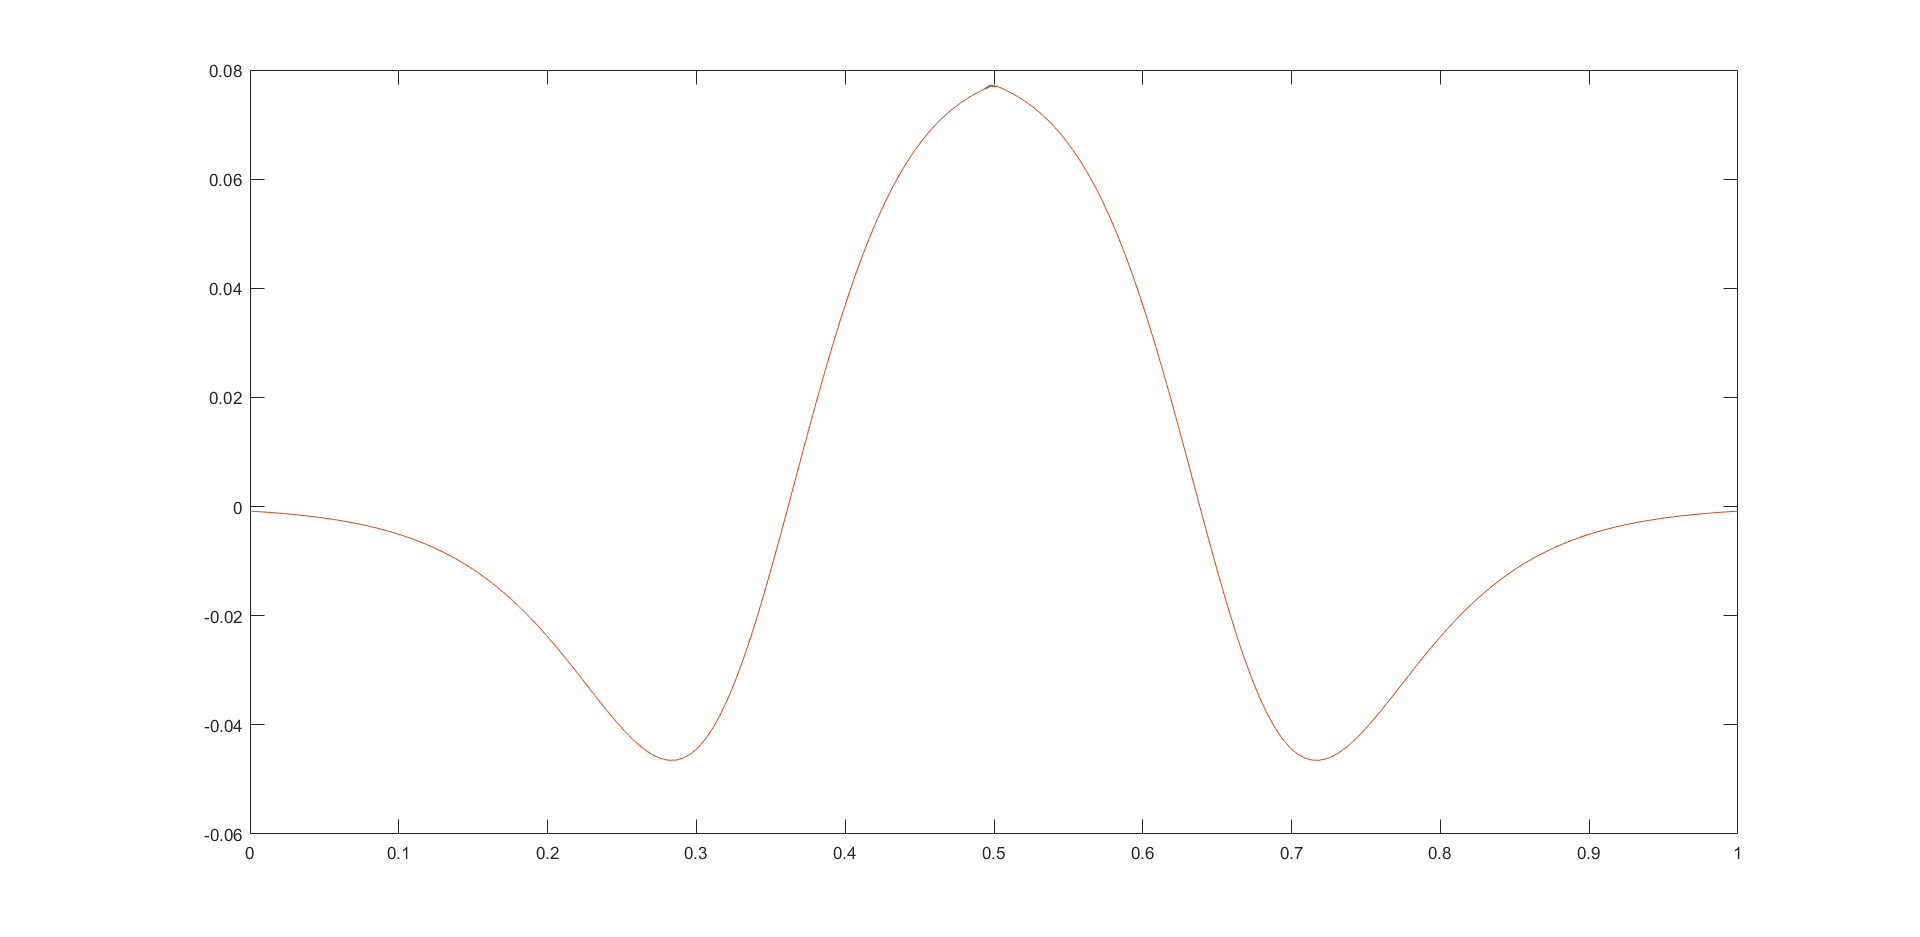
\includegraphics[width=\textwidth]{F.png}
        \caption{$W=0.1$时,$F(y)$的图像(横坐标为$y$方向,纵坐标为$F$的大小)}
    \end{figure}
    }
    \par{数值模拟中,我们将区域$[0,1]\times[0,1]$划分为了
    $200\times 200$个网格点。也即是网格间距为$\triangle x
    =\frac{1}{199}$,时间步长取为$\triangle t=0.1
    \triangle x=\frac{0.1}{199}$。图2为$W=1$算到两时间步
    之间的误差小于$10^{-6}$的图片。图3为$W=0.1$算到达到最大
    迭代步($10^{6}$步)停机的图片
    }
    \begin{figure}[h]
        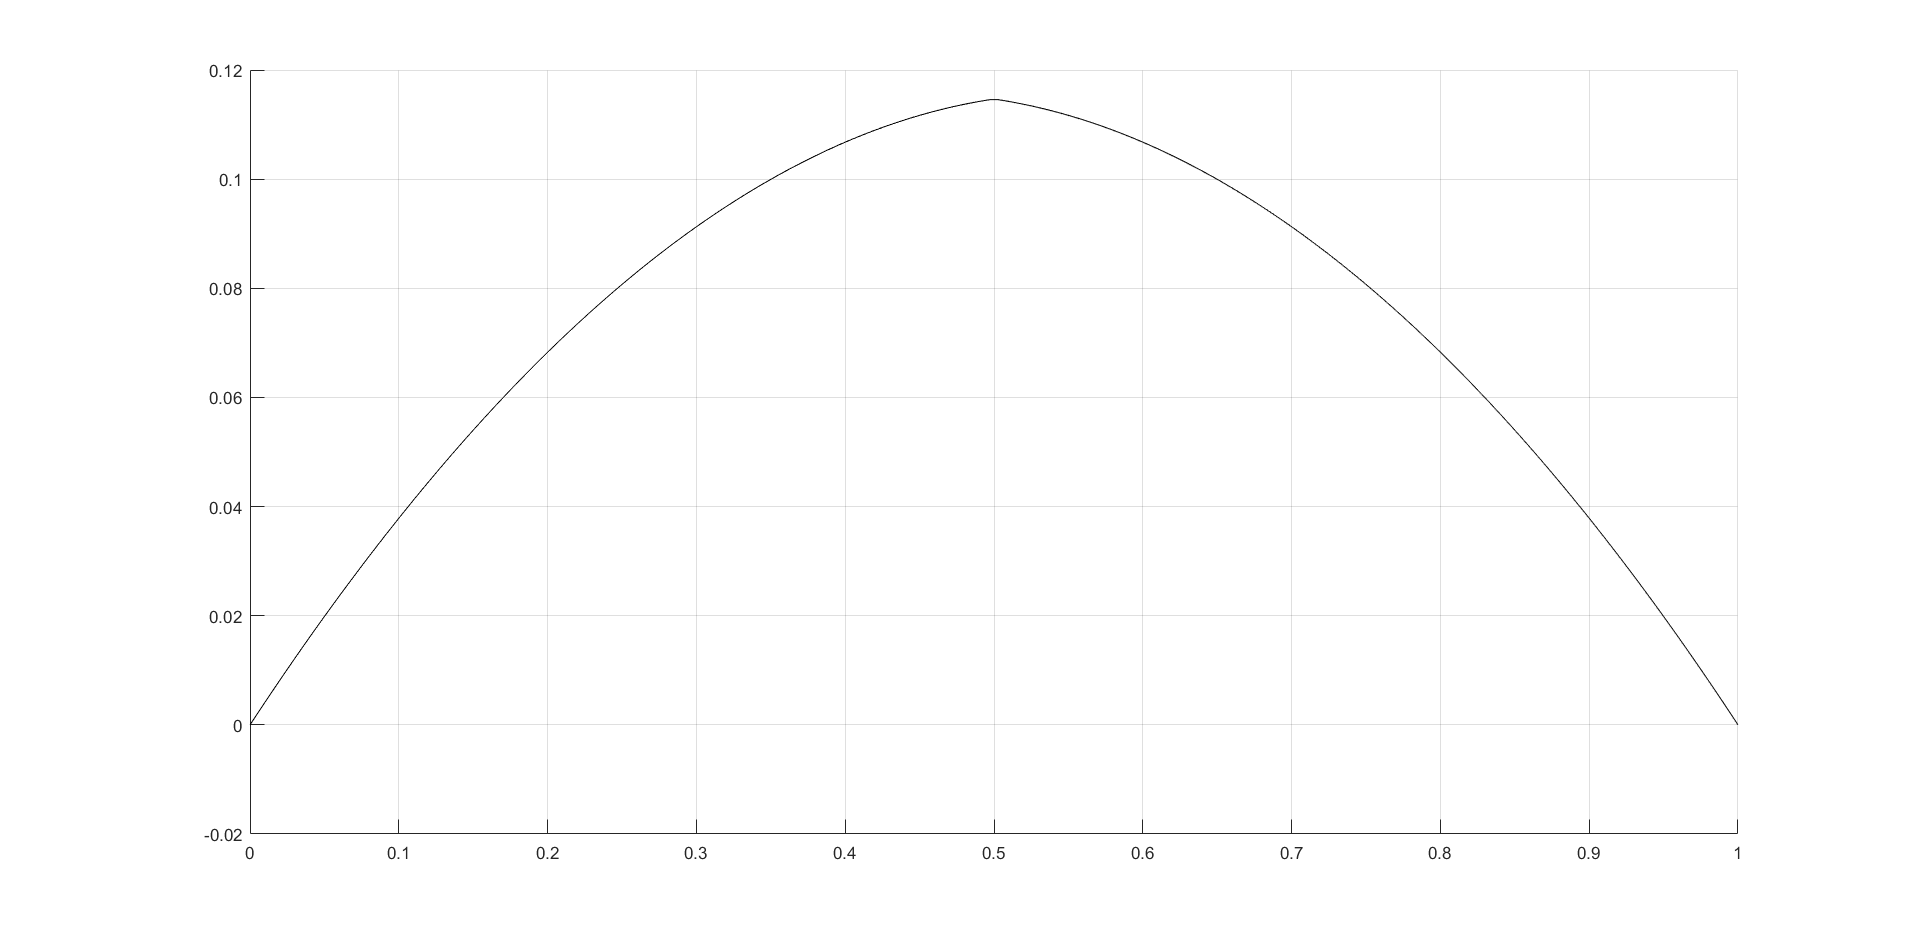
\includegraphics[width=\textwidth]{W=1.png}
        \caption{$W=1$停机后的速度图像(横坐标为$y$方向,纵坐标为$u$的大小)}
    \end{figure}
    \begin{figure}[h]
        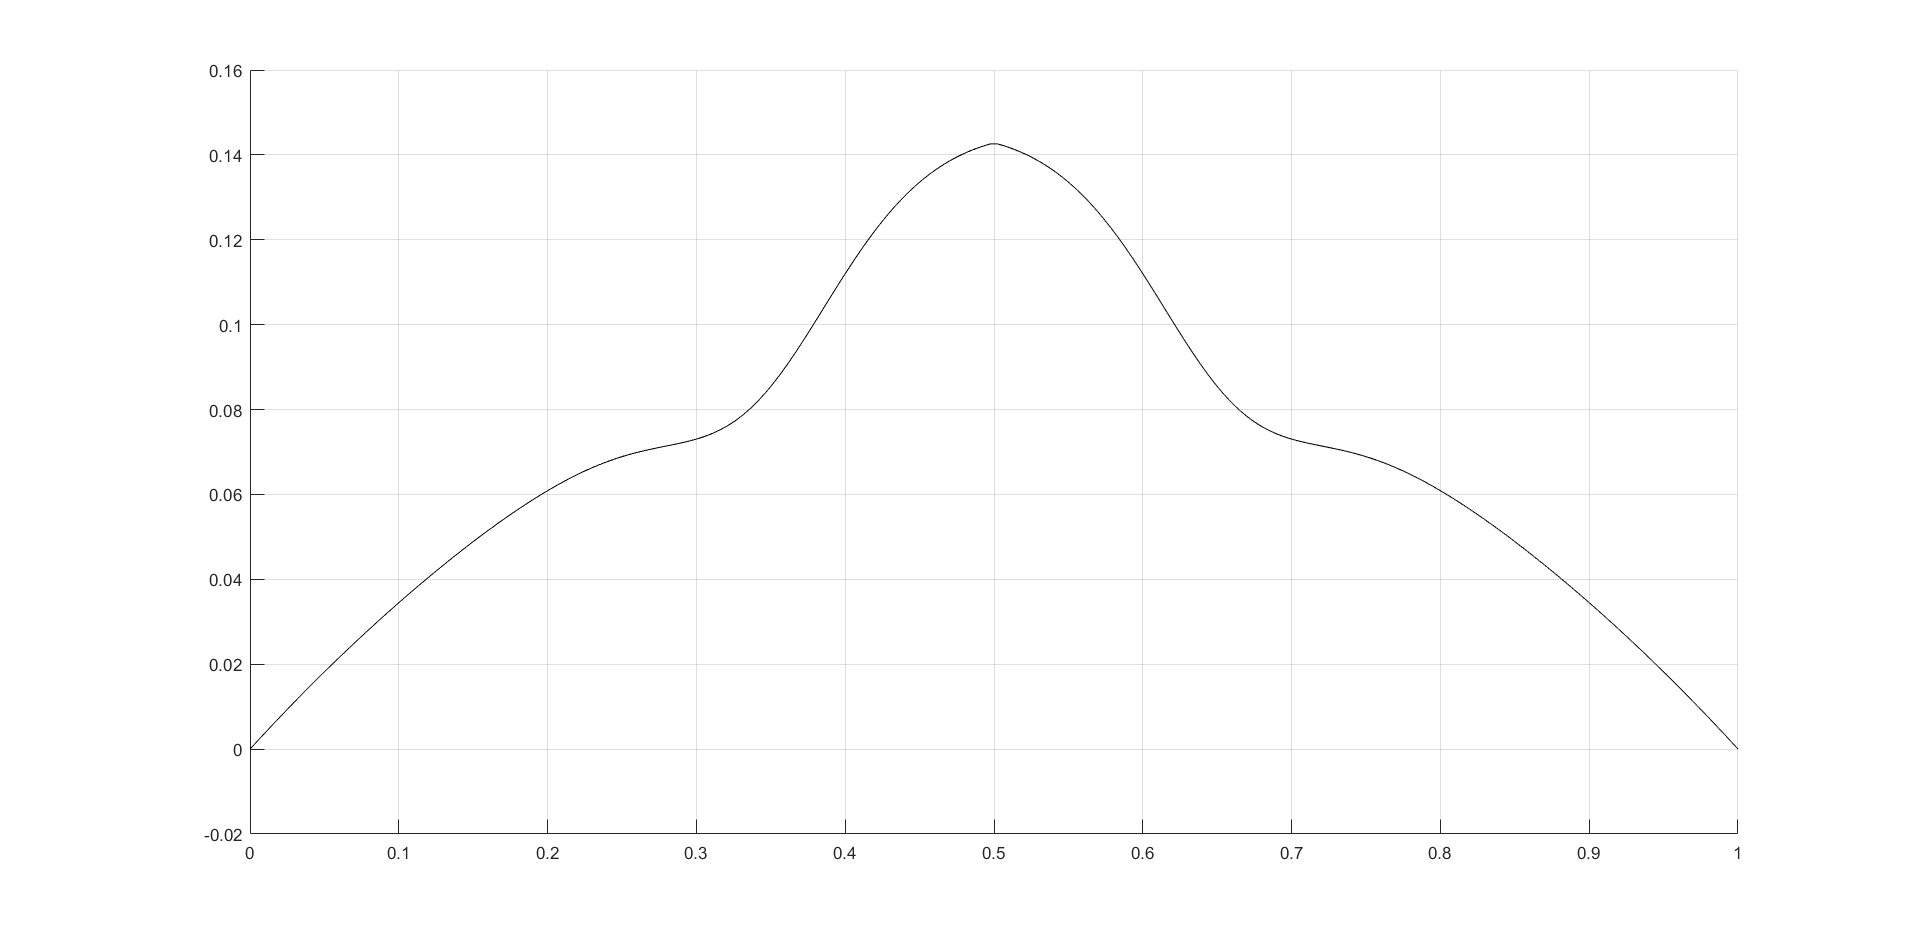
\includegraphics[width=\textwidth]{W=01.png}
        \caption{$W=0.1$停机后的速度图像(横坐标为$y$方向,纵坐标为$u$的大小)}
    \end{figure}
\end{document}